\subsubsection{Funcionalidad y Responsabilidades}

El nivel supervisor constituye la capa de coordinación del sistema, responsable de orquestar tareas complejas que requieren la integración de múltiples subsistemas. A diferencia del nivel regulatorio que ejecuta comandos individuales (mover X milímetros, activar gripper), el supervisor planifica secuencias completas de acciones para lograr objetivos de alto nivel como mapear el entorno o cosechar plantas.

\textbf{Responsabilidades principales:}

\begin{itemize}
    \item \textbf{Planificación de secuencias}: Descompone tareas complejas (ej: "cosechar lechuga en posición X,Y") en secuencias ordenadas de comandos básicos. Determina qué hacer primero, qué condiciones verificar, y cómo responder ante eventos inesperados.

    \item \textbf{Gestión de estado global}: Mantiene información sobre el sistema que el nivel regulatorio no conoce: posición global acumulada desde el homing, dimensiones calibradas del workspace, mapas de ubicaciones de tubos y plantas, y estado del proceso en ejecución. Este estado se actualiza mediante callbacks que procesan mensajes asíncronos del firmware (STEPPER\_MOVE\_COMPLETED, LIMIT\_TRIGGERED).

    \item \textbf{Integración con visión}: Invoca algoritmos de procesamiento de imágenes en momentos específicos de las secuencias, interpreta sus resultados (coordenadas, clasificaciones), y ajusta el plan según lo detectado. Por ejemplo, durante el mapeo decide cuándo capturar imágenes para buscar tubos, y durante la cosecha decide si recolectar una planta según su clasificación morfológica.

    \item \textbf{Comunicación bidireccional}: Envía comandos al nivel regulatorio mediante mensajes UART (formato \texttt{<COMANDO:params>}) y espera respuestas que confirman ejecución exitosa o reportan errores. Actualiza su estado interno según las notificaciones recibidas. Envía señales de sincronización periódicas para que el firmware detecte si el supervisor falló.

    \item \textbf{Persistencia de información}: Guarda datos críticos en archivos JSON que sobreviven reinicios del sistema: referencia de origen tras homing (homing\_reference.json), dimensiones medidas del workspace (workspace\_dimensions.json), última posición conocida (current\_position.json), posiciones Y de tubos detectados (configuracion\_tubos.json), y posiciones X de plantas (matriz\_cintas.json).
\end{itemize}

\textbf{Modelo de ejecución orientado a eventos:}

El supervisor no utiliza hilos concurrentes sino un modelo orientado a eventos mediante callbacks. Cuando envía un comando de movimiento al firmware, no espera bloqueado a que termine. En cambio, registra un callback que será invocado cuando llegue el mensaje \texttt{STEPPER\_MOVE\_COMPLETED}. Durante la espera, el bucle principal del programa continúa procesando otros eventos (mensajes UART entrantes, capturas de cámara). Este diseño evita bloqueos y permite respuesta inmediata a eventos inesperados como activación de finales de carrera.

\subsubsection{Procesos Implementados}

El sistema implementa cuatro procesos principales que coordinan movimientos, captura de imágenes, y ejecución de algoritmos de visión. Cada proceso verifica precondiciones antes de ejecutar acciones críticas (sistema referenciado, brazo en posición compatible, cámara disponible).

\textbf{Proceso 1: Homing (Referenciado del Sistema)}

Establece el origen del sistema de coordenadas moviendo los ejes hasta los finales de carrera y retrocediendo offsets calibrados.

\begin{table}[H]
\centering
\small
\begin{tabular}{|l|p{10cm}|}
\hline
\textbf{Paso} & \textbf{Acción} \\
\hline
1. Verificación inicial & Confirma que el brazo está en posición de movimiento (servos retraídos). Si no lo está, ejecuta transición de brazo antes de continuar. \\
\hline
2. Configuración & Reduce velocidades a HOMING\_SPEED\_H y HOMING\_SPEED\_V (más lentas que velocidades normales para evitar impactos bruscos contra límites). \\
\hline
3. Homing horizontal & Envía comando de movimiento hacia la derecha con distancia muy grande (500mm, mayor que el workspace). El firmware detiene el movimiento al activarse el final de carrera H\_RIGHT. Envía comando de retroceso de HOME\_OFFSET\_H milímetros. \\
\hline
4. Homing vertical & Envía comando de movimiento hacia arriba con distancia muy grande. El firmware detiene al activarse V\_UP. Retrocede HOME\_OFFSET\_V milímetros. \\
\hline
5. Establecer origen & Envía comando \texttt{<XY:0,0>} al firmware para que establezca la posición actual como (0,0). Actualiza el estado global del supervisor a (0,0). \\
\hline
6. Restauración & Restaura velocidades normales (NORMAL\_SPEED\_H, NORMAL\_SPEED\_V). \\
\hline
7. Persistencia & Guarda la referencia en homing\_reference.json con timestamp para verificaciones futuras. \\
\hline
\end{tabular}
\caption{Secuencia del proceso de homing}
\label{tab:proceso_homing}
\end{table}

\textbf{Proceso 2: Calibración del Workspace}

Mide las dimensiones útiles del espacio de trabajo moviendo los ejes hasta sus límites opuestos.

\begin{table}[H]
\centering
\small
\begin{tabular}{|l|p{10cm}|}
\hline
\textbf{Paso} & \textbf{Acción} \\
\hline
1. Homing inicial & Ejecuta proceso de homing para partir desde origen conocido. \\
\hline
2. Medición horizontal & Intenta mover hacia la izquierda una distancia muy grande. El firmware detiene al activar H\_LEFT y envía mensaje de emergencia. El supervisor registra la distancia recorrida como ancho bruto del workspace. \\
\hline
3. Retorno horizontal & Mueve hacia la derecha la distancia registrada más un margen para volver cerca del origen horizontal. \\
\hline
4. Medición vertical & Intenta mover hacia abajo una distancia muy grande. El firmware detiene al activar V\_DOWN. Registra la distancia como alto bruto. \\
\hline
5. Cálculo de dimensiones & Resta márgenes de seguridad (5-10mm) del ancho y alto brutos para obtener dimensiones útiles MAX\_X y MAX\_Y. \\
\hline
6. Homing final & Ejecuta homing nuevamente para volver al origen. \\
\hline
7. Persistencia & Guarda MAX\_X y MAX\_Y en workspace\_dimensions.json. \\
\hline
\end{tabular}
\caption{Secuencia del proceso de calibración}
\label{tab:proceso_calibracion}
\end{table}

\textbf{Proceso 3: Mapeo del Entorno}

Escanea el workspace para detectar posiciones de tubos (coordenadas Y) y plantas (coordenadas X), generando mapas que guían la navegación posterior.

\begin{table}[H]
\centering
\small
\begin{tabular}{|l|p{10cm}|}
\hline
\textbf{Paso} & \textbf{Acción} \\
\hline
1. Escaneo vertical & Desde el origen, mueve el eje vertical hacia abajo en pasos incrementales (ej: cada 5mm). En cada pausa, captura imagen y ejecuta detector de tubos. Si detecta tubo, registra coordenada Y en lista temporal. Continúa hasta recorrer todo el alto del workspace. \\
\hline
2. Guardado de tubos & Ordena las coordenadas Y detectadas de mayor a menor. Las guarda en configuracion\_tubos.json con formato: \texttt{\{"1": \{"y\_mm": 250, "nombre": "Tubo 1"\}, "2": \{...\}\}}. \\
\hline
3. Escaneos horizontales & Para cada tubo en configuracion\_tubos.json: mueve el sistema a la coordenada Y del tubo, ejecuta barrido horizontal desde X=0 hacia la derecha en pasos incrementales, en cada pausa captura imagen y ejecuta detector de cintas, si detecta cinta negra registra coordenada X en lista temporal del tubo. \\
\hline
4. Guardado de cintas & Para cada tubo, guarda las coordenadas X detectadas en matriz\_cintas.json con formato: \texttt{\{"tubo\_1": [50, 120, 190, ...], "tubo\_2": [...]\}}. \\
\hline
5. Retorno & Mueve el sistema de vuelta al origen (0,0). \\
\hline
\end{tabular}
\caption{Secuencia del proceso de mapeo}
\label{tab:proceso_mapeo}
\end{table}

\textbf{Proceso 4: Cosecha Interactiva}

Navega a cada posición registrada en matriz\_cintas.json, clasifica la planta, y si está madura ejecuta la recolección.

\begin{table}[H]
\centering
\small
\begin{tabular}{|l|p{10cm}|}
\hline
\textbf{Paso} & \textbf{Acción} \\
\hline
1. Carga de mapas & Lee configuracion\_tubos.json y matriz\_cintas.json. Valida que existan datos. Genera lista de posiciones (X,Y) a visitar iterando tubos y sus cintas. \\
\hline
2. Navegación & Para cada posición (X,Y): mueve el sistema XY a esa coordenada, espera confirmación de llegada del firmware. \\
\hline
3. Clasificación & Captura imagen con la cámara. Ejecuta clasificador morfológico que retorna: clase predicha (LECHUGA, PLANTIN, VASO\_VACIO, etc.) y confianza (0-1). \\
\hline
4. Decisión & Si clase es LECHUGA: ejecuta corrección de posición con detectores de cintas para centrar la planta bajo el gripper (ajustes de ±10mm típicamente), transfiere el brazo de posición "movimiento" a "recoger" (servos se extienden hacia planta), envía comando de cierre del gripper, espera confirmación GRIPPER\_CLOSED, transfiere brazo a posición "transportar" (eleva planta). \\
\hline
5. Depósito & Si tiene planta en gripper: navega a zona de depósito (coordenadas predefinidas cerca de un borde), transfiere brazo a posición "depositar" (inclina hacia contenedor), abre gripper, espera confirmación GRIPPER\_OPENED, transfiere brazo a "transportar". \\
\hline
6. Continuación & Si quedan posiciones por procesar, vuelve al paso 2. Si no, procede al paso 7. \\
\hline
7. Finalización & Navega de vuelta al origen (0,0). Transfiere brazo a posición "movimiento". Registra estadísticas: plantas cosechadas, vasos vacíos, plantas inmaduras. \\
\hline
\end{tabular}
\caption{Secuencia del proceso de cosecha interactiva}
\label{tab:proceso_cosecha}
\end{table}

\textbf{Manejo de errores durante procesos:}

Durante la ejecución de cualquier proceso, el supervisor monitorea eventos inesperados:

\begin{itemize}
    \item \textbf{Límite activado inesperadamente}: Si recibe LIMIT\_TRIGGERED durante un movimiento que no debería alcanzar límites, detiene el proceso, registra el error, y preserva el estado para diagnóstico.
    \item \textbf{Pérdida de comunicación}: Si un comando no recibe respuesta en tiempo límite configurado (ej: 30s para movimientos largos), aborta el proceso e intenta re-establecer comunicación.
    \item \textbf{Fallo de detector}: Si un algoritmo de visión no retorna resultados válidos (ej: no detecta tubo esperado), registra la falla e intenta continuar con la siguiente posición, o solicita intervención del usuario según la severidad.
\end{itemize}

\begin{figure}[H]
    \centering
    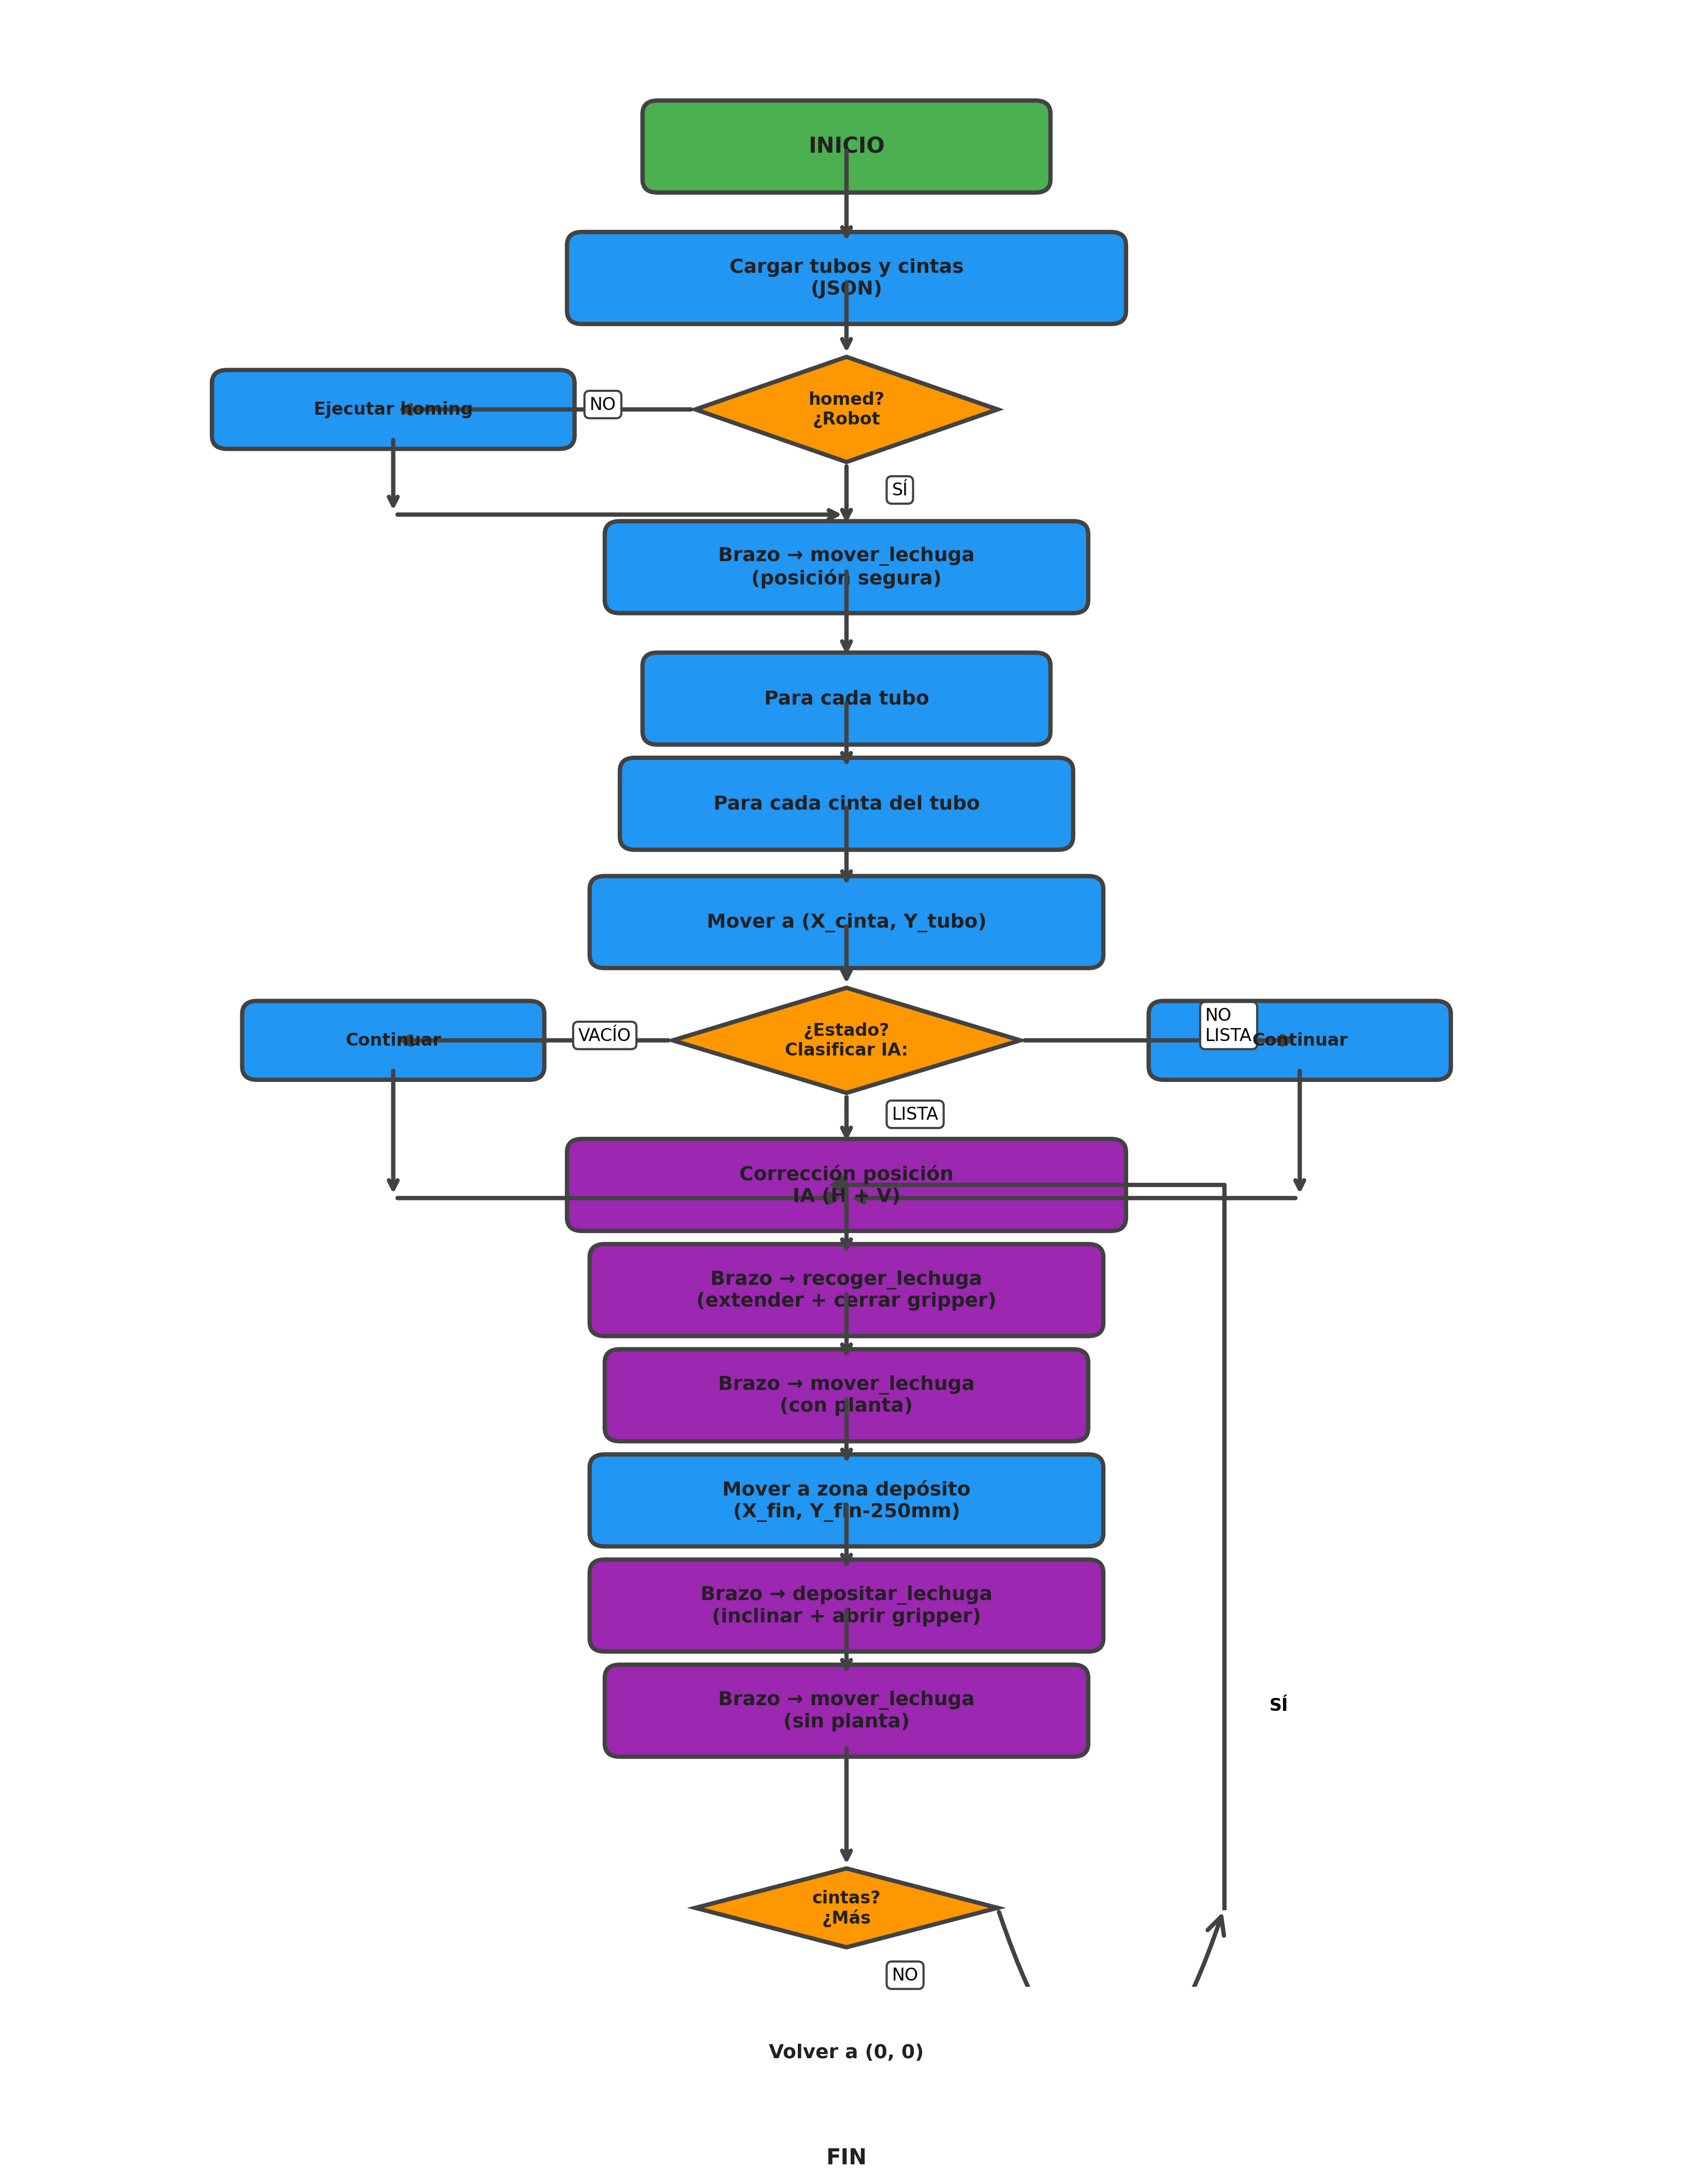
\includegraphics[width=0.85\textwidth]{imagenes/diagrama_flujo_cosecha.png}
    \caption{Diagrama de flujo detallado del proceso de cosecha mostrando decisiones según clasificación}
    \label{fig:flujo_cosecha}
\end{figure}
